% absolutely incredible document format made by yours truly
% - Jorn Veken, 2022
\documentclass{article}
\usepackage[dutch]{babel}
\usepackage{float}
\usepackage{mwe}
\usepackage[hidelinks,breaklinks]{hyperref}

\usepackage{csquotes}
\usepackage[sorting=none]{biblatex}
% \bibliography{bronnen.bib}

% Remove this in your fork if you are cool
\usepackage{lipsum}

% Yea, I got a bunch of custom styling, stored in ./style/ . It's all pretty, self explanatory.
% absolutely incredible document format made by yours truly
% - Jorn Veken, 2022
\usepackage{xcolor}
\usepackage{fontspec}
\usepackage[a4paper, total={6in, 8in}]{geometry}
\usepackage{multicol}

% Background style
\definecolor{page_bg}{rgb}{1.0, 1.0, 1.0}
\pagecolor{page_bg}

% Foreground style
\definecolor{page_fg}{rgb}{0.1, 0.1, 0.1}

\defaultfontfeatures{RawFeature={+axis={wght=100}}}
\setmainfont[
    Path = ./style/fonts/, 
    UprightFont = *-Regular,
    BoldFont = *-Bold,
    ItalicFont = *-Italic,
    ]
{MainFont}

% Default text style
\color{page_fg}
% absolutely incredible document format made by yours truly
% - Jorn Veken, 2022
% Headers and footer definitions
% Include before document begin

\usepackage{fancyhdr}
\pagestyle{fancy}
\fancyhf{}

% Header
\lhead{Jorn Veken}
\rhead{Pagina \thepage}

% Footer
\rfoot{\today}
\lfoot{Lectoraat Smart Driven Data Society \& Inholland Alkmaar}
% absolutely incredible document format made by yours truly
% - Jorn Veken, 2022
% Definitions for code blocks
% Include document begin
\usepackage{listings}
\usepackage{xcolor}
\usepackage{fontspec}
\usepackage[most]{tcolorbox}

% Load code font
\setmonofont[
    Path = ./style/fonts/, 
    UprightFont = *-Regular,
    BoldFont = *-Bold,
    ItalicFont = *-Italic,
    ]
{Codeblock}

% Basic
\definecolor{color_bg}{rgb}{1.0, 1.0, 1.0}
\definecolor{color_fg}{rgb}{0.2, 0.2, 0.2}

% Keywords
\definecolor{color_comment}{rgb}{0.5, 0.3, 1.0}
\definecolor{color_keyword}{rgb}{1.0, 0.3, 0.5}
\definecolor{color_string}{rgb}{0.8, 0.4, 0.4}

% Codeblock specific
\definecolor{color_linenum}{rgb}{0.3, 0.3, 0.3}

% Style definition
\lstdefinestyle{codeblock_default}{
    backgroundcolor = \color{color_bg},   
    commentstyle    = \it\color{color_comment},
    keywordstyle    = \bf\color{color_keyword},
    numberstyle     = \bf\tiny\color{color_linenum},
    stringstyle     = \color{color_string},
    basicstyle      = \small\ttfamily\color{color_fg},
    % Spacing
    breakatwhitespace = false,
    breaklines  = true,                 
    captionpos  = b,                    
    keepspaces  = true,                 
    numbers     = left,                    
    numbersep   = 5pt,                  
    showspaces  = false,        
    % Tabs and Space visibility
    showstringspaces = false,
    showtabs = false,                  
    tabsize  = 2
}

% Set style
\lstset{style=codeblock_default}

\newcommand\titletext{Modelleren UML}
\newcommand\authortext{Luc Appelman (640696@student.inholland.nl)}

\title{\LARGE{\titletext}\\\normalsize{Beschrijving van de klassen voor de SenseBox}}
\author{\authortext}
\date{\today}

% color links and pdf info
\hypersetup{
  colorlinks=true, % color links instead of border
  linkcolor=blue!50!black,
  urlcolor=blue!50!black,
  citecolor=blue!50!black,
  pdftitle={\titletext},
  pdfauthor={\authortext},
  breaklinks=true
}

\newcommand{\contents} {
  {
    \hypersetup{hidelinks}
    \tableofcontents
  }
  \clearpage
}

\begin{document}

    % This is the first page of the document
    % --------------------------------------
    \maketitle
    % \vspace{8em}
    % \begin{figure}[H]
    %     \centering
    %     \includegraphics[width=30em, height=20em]{example-image-a}
    %     \caption[lettertje]{GROTE LETTER A}
    % \end{figure}
    \vfill
    \newpage
    % --------------------------------------

    % Inhoudsopgave
    \contents

    % To use codeblocks, write \begin{codeblock} \end{codeblock}
    % absolutely incredible document format made by yours truly
% - Jorn Veken, 2022
\newtcblisting{codeblock}[2][]{%
    enhanced, title=#2, 
    colback=white,
    attach boxed title to top left = {xshift=5mm,yshift=-2mm},
    fonttitle=\ttfamily, coltitle=white,
    listing only,listing options={language=C, basicstyle=\ttfamily\footnotesize},#1}

% Here's a code snippet for code blocks.
\iffalse
begin{codeblock}{main.py}
   import cv2 as cv
   
   def main()
       print('Hello, world!')
       return
   
   if __name__ == '__main__' :
       main()
\end{codeblock}
\fi

    % Here all the sections go. Stored in ./sections/
    % --------------------------------------
    \begin{flushleft}
    % Multicol maakt van die mooie kolommen.
    \section{Abstract}
\textbf{\lipsum[1]}

\section{Inleiding}
\lipsum[2]

\vspace{1em}
\lipsum[3-4]\cite{lorem}

    \newpage
    \section{Modellen}

    \subsection{Sensoren}
\subsubsection{Klassendiagram}
Het doel van de klassen die de sensoren uitlezen is om een structuur op te zetten waarbij zo gemakkelijk mogelijk nieuwe sensoren vervangen/toegevoegd kunnen worden. Ook is het van belang dat van buiten af voor het meten van alle sensoren maar één functie aangeroepen hoeft worden. Hierom is er voor gekozen om de zogeheten CSensorManager aan te maken. Dit is een singleton omdat er altijd maar één manager aangemaakt mag worden in het programma. Aan deze manager kunnen een x aantal sensoren toegevoegd worden.
\vspace{1em}
Wanneer de \emph{mMeasure()} member aangeroepen wordt zal iedere sensor uitgemeten worden. Het resultaat van iedere sensor is beschreven in een SensorOutput map. Deze worden gecombineerd in het Measurements datatype, dit wordt door de \emph{mMeasure()} functie.
\vspace{1em}
Om ieder type sensor te ondersteunen is er een \emph{CSensor} klasse aangemaakt die de minimale functionaliteit van iedere sensor beschrijft, een daadwerkelijke sensor klasse erft deze klasse en kan toegevoegd aan de sensor manager. De \emph{m\_InitCallback()} en \emph{m\_MeasureCallback()} members zijn virtual en worden gebruikt om de sensor specifieke functies van een sensor te implementeren. Iedere \emph{CSensor} heeft ook een \emph{m\_Status} property van het type \emph{CSensorStatus} waarin de status van de sensor opgeslagen is.

\begin{figure}[H]
  \centering
  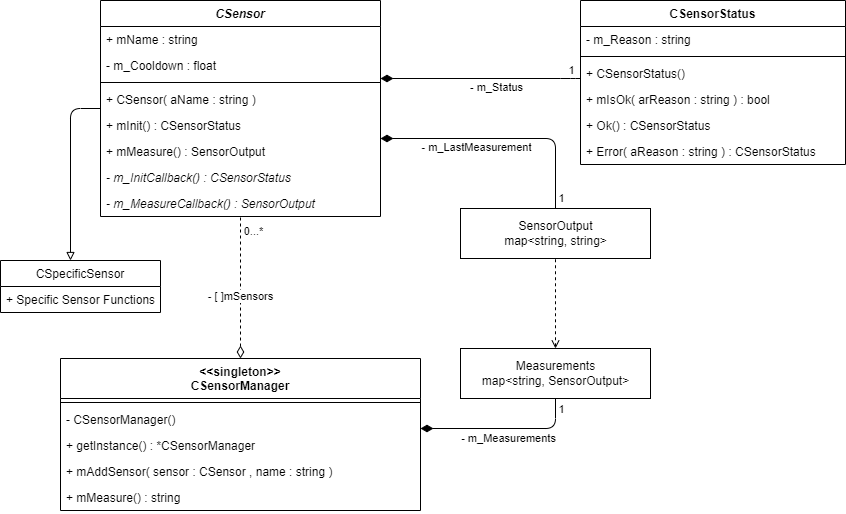
\includegraphics[width=\columnwidth]{uml/sensor-abstraction.png}
\end{figure}

\newpage
\subsubsection{Toestandsdiagram}
De klassen hebben een aantal states waarin de klasse kan verblijven. Over de grootste tijd zullen ze in de idle state staan omdat we slechts één keer per minuut meten. Het meten kan alleen gedaan worden als er al een sensor toegevoegd is aan de sensor manager. Het initialiseren van een sensor gebeurt buiten de sensor manager, een sensor mag alleen toegevoegd worden als de status van de status geen error is.
\vspace{1em}
Het meten van een sensor mag één keer fout gaan, hierdoor wordt er ook een warning in de log opgeschreven. Als hierna het meten van de sensor weer niet goed gaat zal er een error opgeslagen worden in de sensor klasse. Deze status zal later uitgelezen en gelogd moeten worden voordat de metingen opgestuurd worden naar het IoT platform.
\vspace{1em}
Het opslaan van de gemeten waarden kan op twee manieren. Bij voorkeur gaat dit via een bericht met alle getemeten waarden over het internet zodat de waarden direct in het IoT platform staan. Mocht de SenseBox geen actieve internet verbinding hebben wordt de data alsnog in een log bestand op de interne SD kaart opgeslagen zodat deze informatie later alsnog uitgelezen kan worden.

\begin{figure}[H]
  \centering
  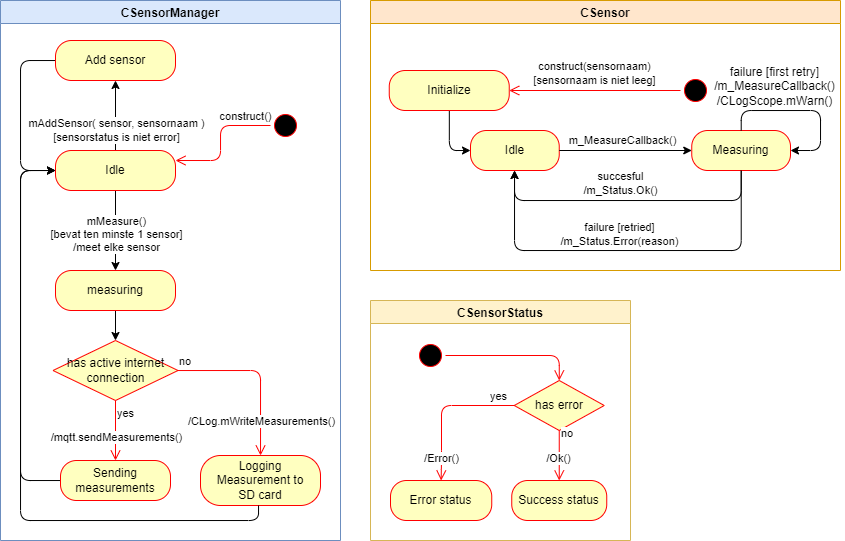
\includegraphics[width=\columnwidth]{uml/sensor-state-diagram.png}
\end{figure}
    \newpage
\subsection{WiFi verbinding}
\subsubsection{Klassendiagram}
Om de verzamelde informatie te versturen wordt er gebruik gemaakt van een WiFi verbinding die aangemaakt wordt wanneer de SenseBox opstart. Dit is ook een singleton omdat er maar één wifi antenne is en er dus maar met één netwerk tegelijk verbinding gemaakt kan worden. Het ip address wordt opgeslagen in de klasse zodat deze later opgevraagd kan worden buiten de klasse. Bij het aanmaken van een WiFi verbinding moeten de inloggegevens voor het netwerk meegegeven worden in de constructor.

\begin{figure}[H]
  \centering
  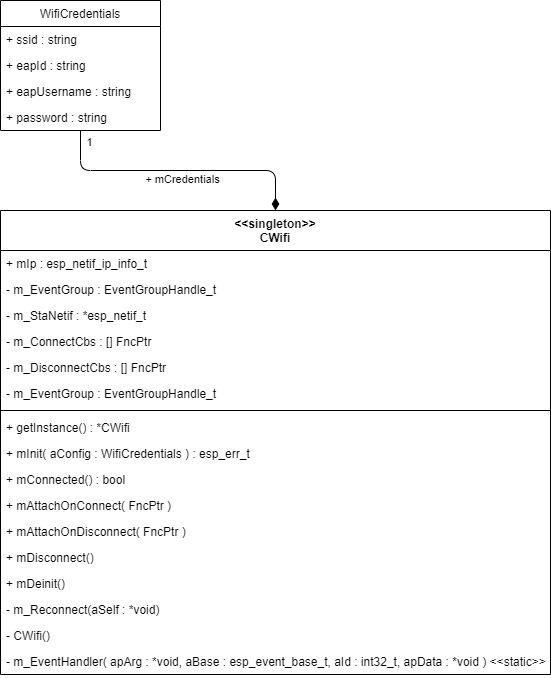
\includegraphics[width=.6\columnwidth]{uml/wifi-network-stack.png}
\end{figure}

\newpage
\subsubsection{Toestandsdiagram}
Wanneer de WiFi verbinding gestart wordt moeten de inloggegevens meegegeven worden met de constructor. Als de EAP gebruikersnaam hierin niet leeg is weten we dat we met een WPA2 Enterprise netwerk willen verbinden, dit is nodig om met het netwerk op school te kunnen verbinden. Als de gebruikersnaam leeg is moet er verbonden worden met een normaal WPA2 netwerk zoals je dat thuis hebt. Vanuit de WiFi verbinding kunnen er verschillende events gegenereerd worden die opgevangen moeten worden door de \emph{m\_EventHandler} member functie. Als dit gebeurt wordt de status van de verbinding bijgewerkt.
\vspace{1em}
Omdat er gebruik gemaakt wordt van FreeRTOS kunnen andere functies van FreeRTOS direct gebruik maken van de WiFi verbinding zonder dat hiervoor een speciale write of read functie aangemaakt moet worden. Dit is dan ook niet opgenomen in de toestandsdiagram.

\begin{figure}[H]
  \centering
  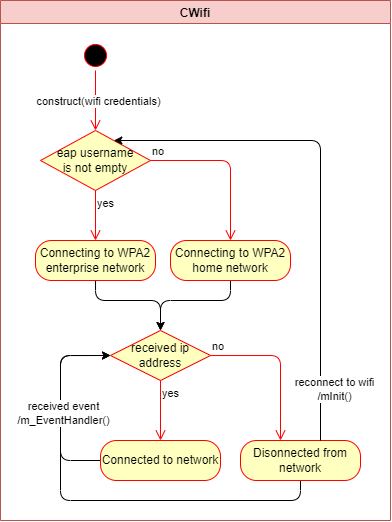
\includegraphics[width=.45\columnwidth]{uml/wifi-state-diagram.png}
\end{figure}
    \newpage
\subsection{Log systeem}
\subsubsection{Klassendiagram}
Om informatie over het programma op te slaan terwijl er metingen etc. gedaan worden kan er informatie naar één van de drie log bestanden geschreven worden. Er worden in totaal drie logbestanden bijgehouden: \emph{m\_Measurements}, \emph{m\_Log} en \emph{m\_Debug}. Er is een enum voor het type log dat we willen schrijven, in de implementatie zal hiervoor dan een herkenbare tag als prefix gezet worden voor de log entry. Er wordt ook gebruik gemaakt van een log scope, deze wordt gebruikt om aan te geven welk onderdeel van het programma iets naar het log geschreven heeft. Een scope zal een zelfde soort tag krijgen als het logtype.

\begin{figure}[H]
  \centering
  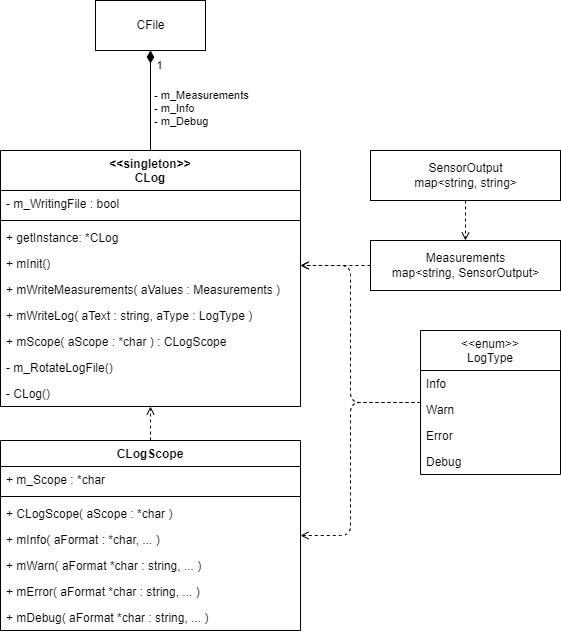
\includegraphics[width=.7\columnwidth]{uml/logger-abstraction.png}
\end{figure}

\newpage
\subsubsection{Toestandsdiagram}
Een nieuwe regel kan aan het log toegevoegd worden via twee verschillende functies. \emph{mWriteMeasurements()} en \emph{mWriteLog()}, de eerste hiervan wordt gebruikt om naar het log bestand in \emph{m\_Measurements} te schrijven wanneer er geen actieve internet verbinding is. De tweede kan zowel naar \emph{m\_Log} en \emph{m\_Debug} schrijven, afhankelijk van het \emph{LogType} dat wordt meegegeven in de functie. De \emph{LogType} wordt bepaald door de functie die wordt aangeroepen in \emph{CLogScope}.
\vspace{1em}
Wanneer er geen SD kaart in de SenseBox zit wordt dit verwerkt in de \emph{CFile} klasse en zal dit niet zorgen voor problemen in de \emph{CLog} klasse.

\begin{figure}[H]
  \centering
  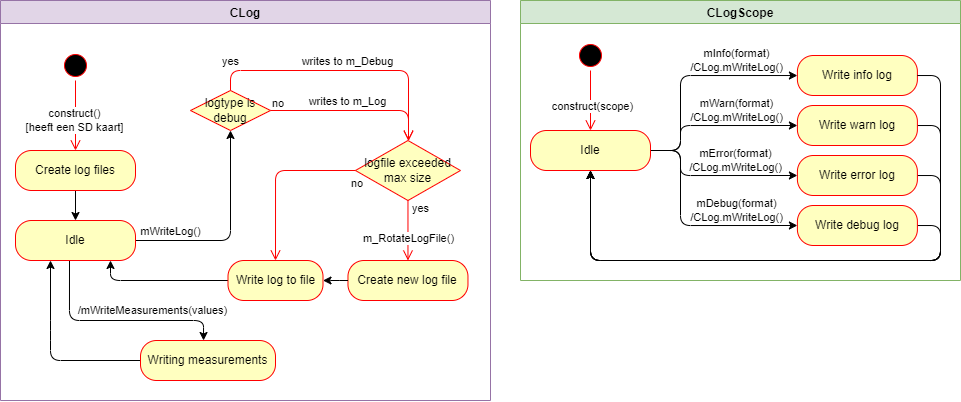
\includegraphics[width=\columnwidth]{uml/logger-state-diagram.png}
\end{figure}
    \end{flushleft}
    % --------------------------------------
    
    \newpage
    % Sources at the end
    % \printbibliography

\end{document} % This is the end of the document